\section{Data} \label{sec:data}
This study employs two complementary datasets covering the period from January 1, 2020 to December 31, 2024: daily Bitcoin spot prices for physical measure estimation and intraday Deribit BTC inverse option transaction records for risk-neutral measure calibration. The analysis presented here focuses on the 2024 subsample for illustrative purposes, as it encompasses the most liquid and eventful period in the sample.\todo{To be determined what period(2020$\sim$2024 or only 2024) to show}

\subsection{Bitcoin Spot Prices and Log Returns}
Bitcoin spot prices are sourced at daily frequency and exhibit a pronounced bull market throughout 2024, rising from approximately \$40,000 at the start of the year to a peak exceeding \$106,000 in late November before retracing to approximately \$93,000 by year-end (Figure 1, left panel). This appreciation was driven by two structural catalysts: the approval of spot Bitcoin ETFs in the United States in January 2024 and the fourth Bitcoin block reward halving in April 2024, both of which materially shifted the supply-demand balance and attracted substantial institutional inflows.

\begin{figure}[h]
    \centering
    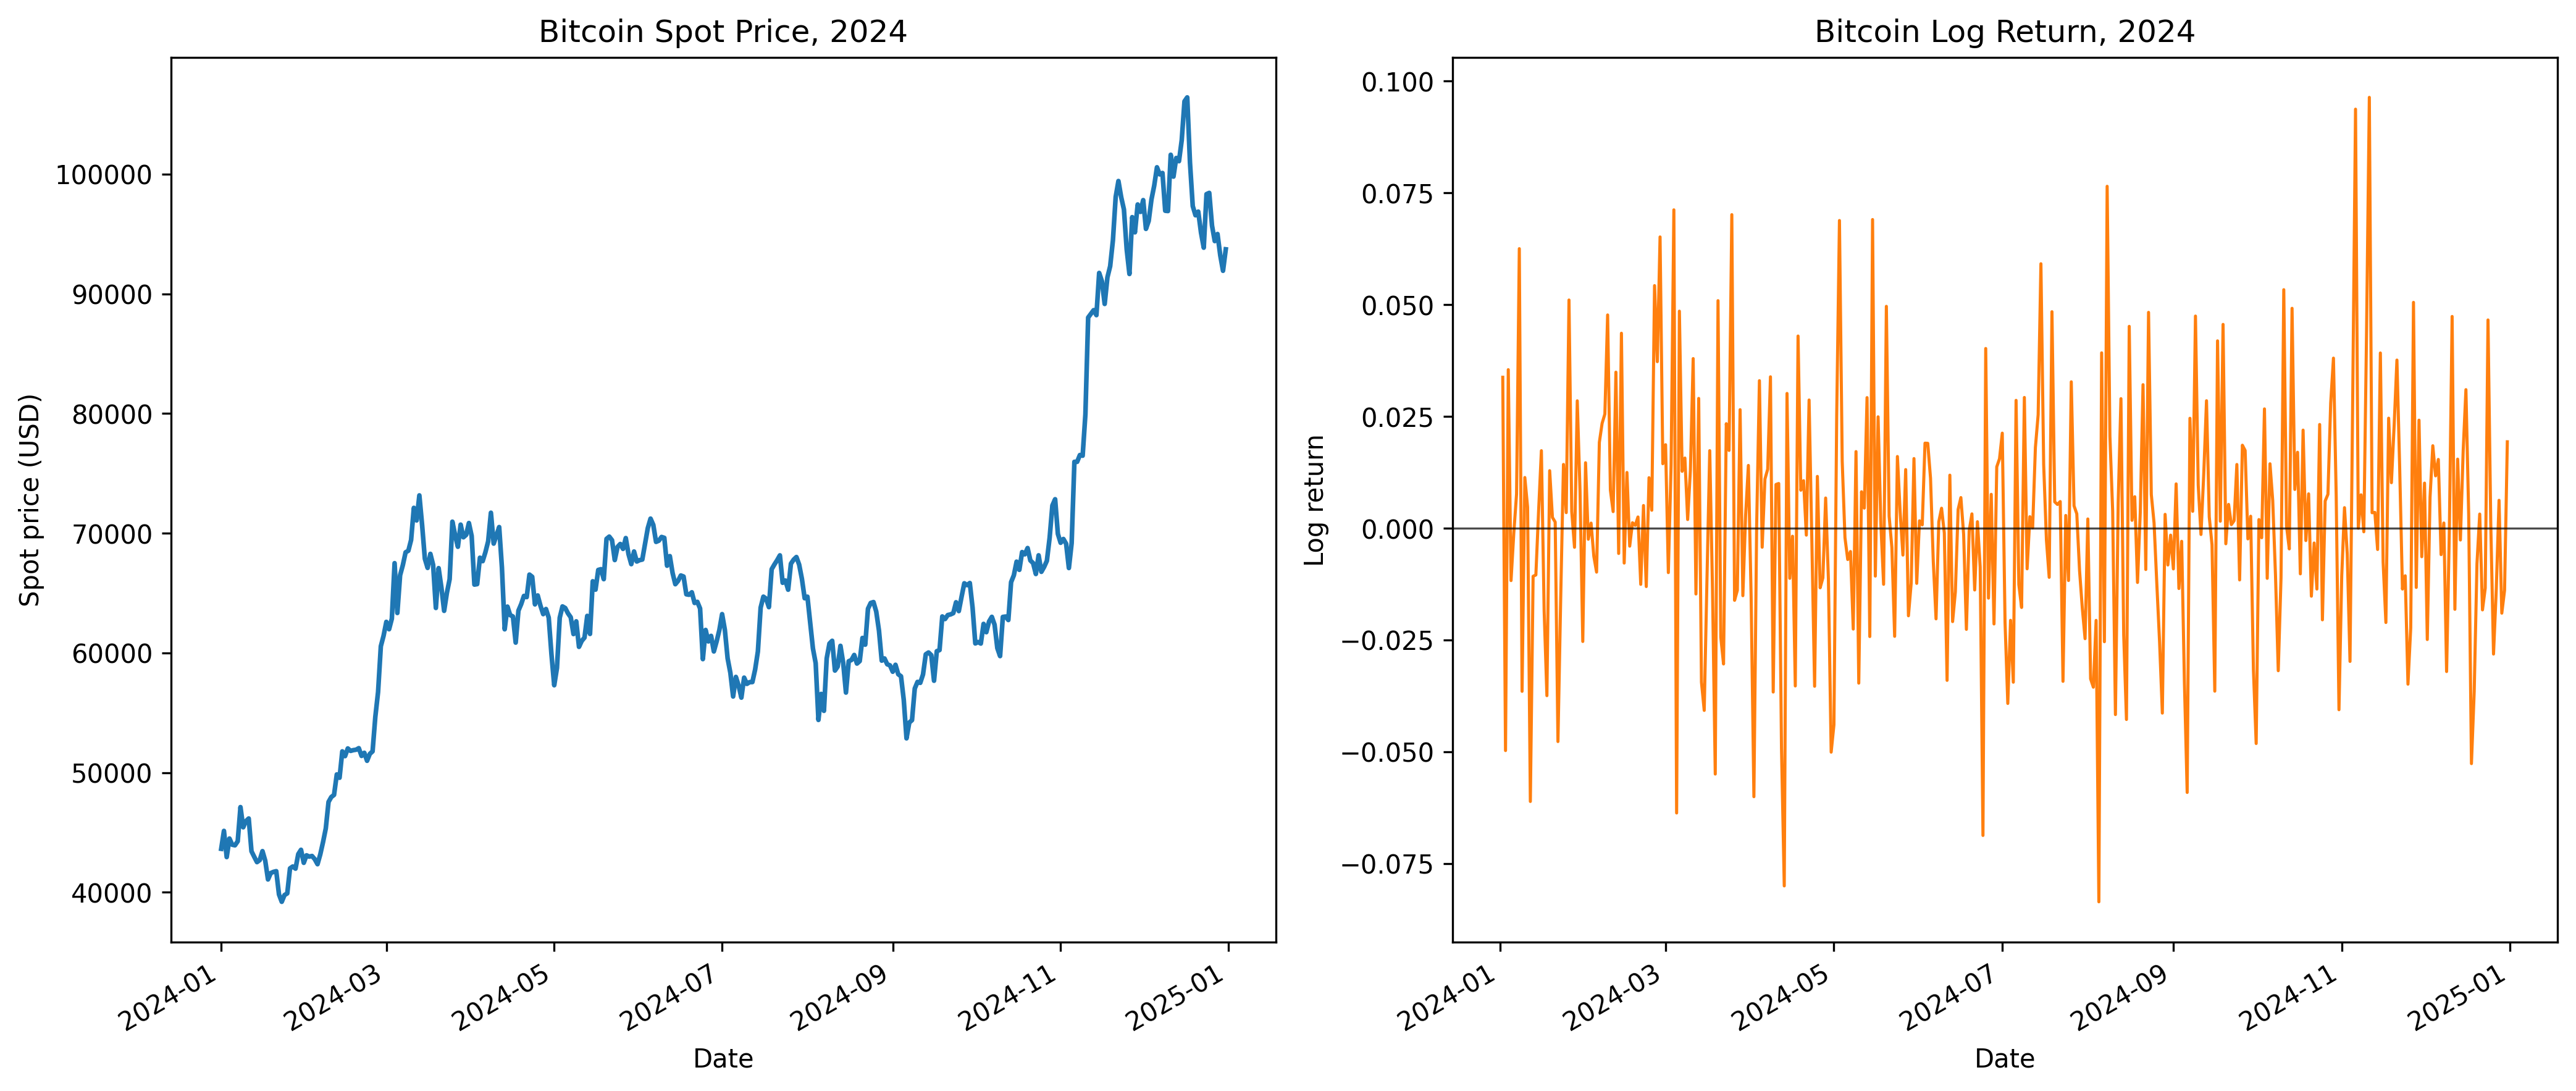
\includegraphics[width=\linewidth]{Sections/02_data_figures/btc_spot_and_log_return_2024.png}
    \caption{Bitcoin spot and log return time series for 2024}
    \label{fig:placeholder}
\end{figure}

The corresponding daily log return series (Figure 1, right panel) reveals the key distributional features that motivate the SVCJ modeling framework adopted in this thesis. As reported in Table 1, descriptive statistics for daily Bitcoin log returns over the full sample period from 2014 to 2024. The mean daily return of 0.001371 corresponds to an annualized return of approximately 50\%, yet the near-zero median of 0.000000 reveals that this long-run appreciation is driven by a small number of extraordinary return days rather than steady drift — a hallmark of a jump-driven process. The standard deviation of 0.034990 implies an annualized volatility of approximately 67\%, reflecting the repeated boom-and-bust cycles that characterize the decade, including the 2017–2018 crash, the March 2020 COVID collapse, and the 2021–2022 drawdown exceeding 70\%.

The distributional shape departs dramatically from normality along both dimensions of the Jarque-Bera decomposition. Skewness of -0.427 indicates a pronounced left tail: the largest single-day loss of -31.7\% substantially exceeds the largest single-day gain of +19.1\% in magnitude, reflecting crash episodes that pull the distribution asymmetrically downward and generate a downside jump risk premium embedded in Bitcoin option prices. Kurtosis of 9.754 — more than three times the Gaussian benchmark of 3 — confirms that extreme return realizations occur far more frequently than any normal distribution would predict. Jointly, these features produce a Jarque-Bera statistic of 7,527.47, constituting a categorical rejection of normality at any conventional significance level and closing the door on Black-Scholes as a viable pricing framework. These distributional facts collectively motivate the SVCJ specification adopted in this thesis, which explicitly accommodates stochastic volatility, correlated price jumps, and correlated volatility jumps as the minimum viable structure for capturing Bitcoin's return dynamics.

\begin{table}[h]
    \centering
    \begin{tabular}{cc}
    \hline
    \multicolumn{2}{c}{Descriptive statistics} \\
    \hline
        Mean & 0.001371 \\
        Standard deviation & 0.034990\\
        Skewness & $-0.426816$\\
        Kurtosis & 9.7541098\\
        Minimum & $-0.317282$\\
        Median & 0.000000\\
        Maximum & 0.190903\\
        JB & 7527.471506\\
        \hline
    \end{tabular}
    \caption{Descriptive statistics of Bitcoin log return (2014 to 2024)}
    \label{tab:placeholder}
\end{table}

\subsection{Deribit BTC Inverse Options and Daily Closing Prices}
\label{subsec:deribit_filtered_options}

The options dataset consists of intraday transaction records for European-style BTC inverse options traded on Deribit, the dominant venue for Bitcoin option trading. Inverse options are denominated and settled in Bitcoin rather than US dollars, so the BTC-denominated payoff differs from the payoff of a standard USD-settled option. This payoff convention is retained throughout the empirical analysis because the risk-neutral calibration is performed in the original BTC price units observed in the market.

Daily risk-neutral calibration requires a cross-section of option prices that refers, as closely as the data permit, to a common valuation time. Pooling all transactions over a 24-hour trading day would mix contracts traded under different intraday spot prices, volatility states, and remaining maturities. We therefore anchor each daily cross-section at 08:00 UTC, the natural Deribit settlement and option-expiration time. Because exact 08:00 transaction prices are generally unavailable, we construct a transaction-based closing panel from actual regular outright trades observed in a short interval centered on 08:00 UTC.


\begin{figure}[h]
    \centering
    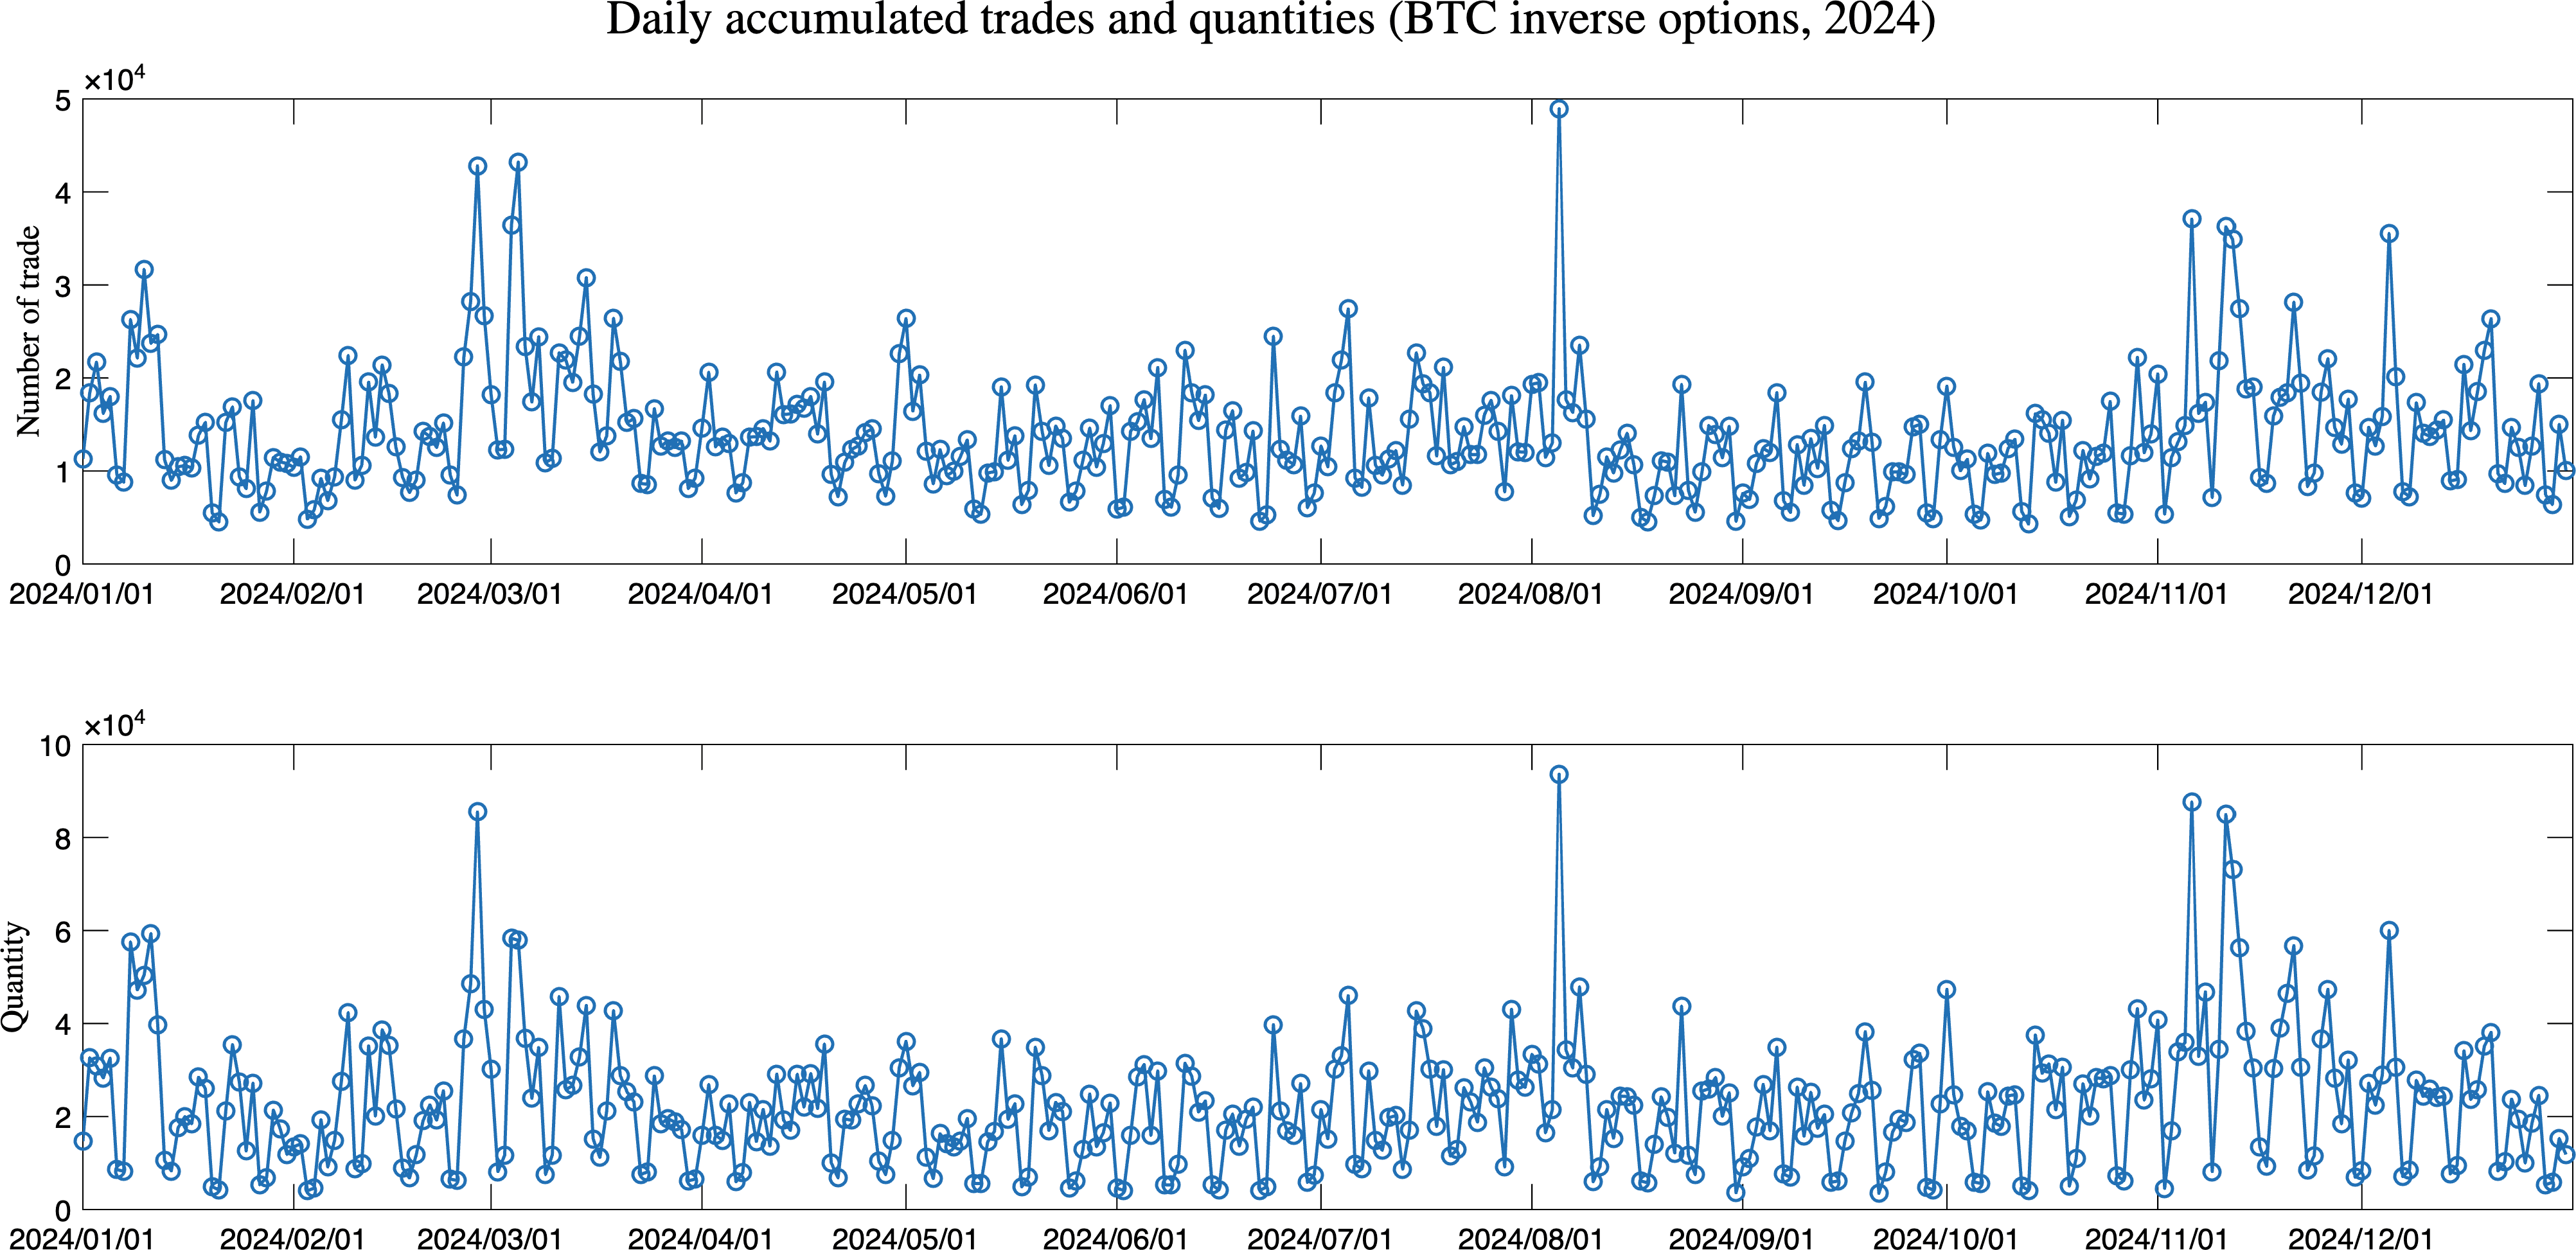
\includegraphics[width=\linewidth]{Sections/02_data_figures/Daily_traded_quantity.png}
    \caption{Daily accumulated trades and quantities}
    \label{fig:2024_daily_accu_trades_and_q}
\end{figure}

Figure~\ref{fig:2024_daily_accu_trades_and_q} shows daily trading activity throughout 2024, with the number of trades fluctuating between approximately 5,000 and 45,000 per day and total daily quantity ranging between 5,000 and 90,000 BTC notional. Two prominent spikes in both trades and quantity are visible around late February to early March and late July to early August 2024, coinciding with periods of elevated Bitcoin price volatility and heightened hedging demand. The overall level of activity confirms that the Deribit market is sufficiently liquid to support the daily cross-sectional calibration undertaken in this thesis.

\clearpage

\begin{figure}[h]
    \centering
    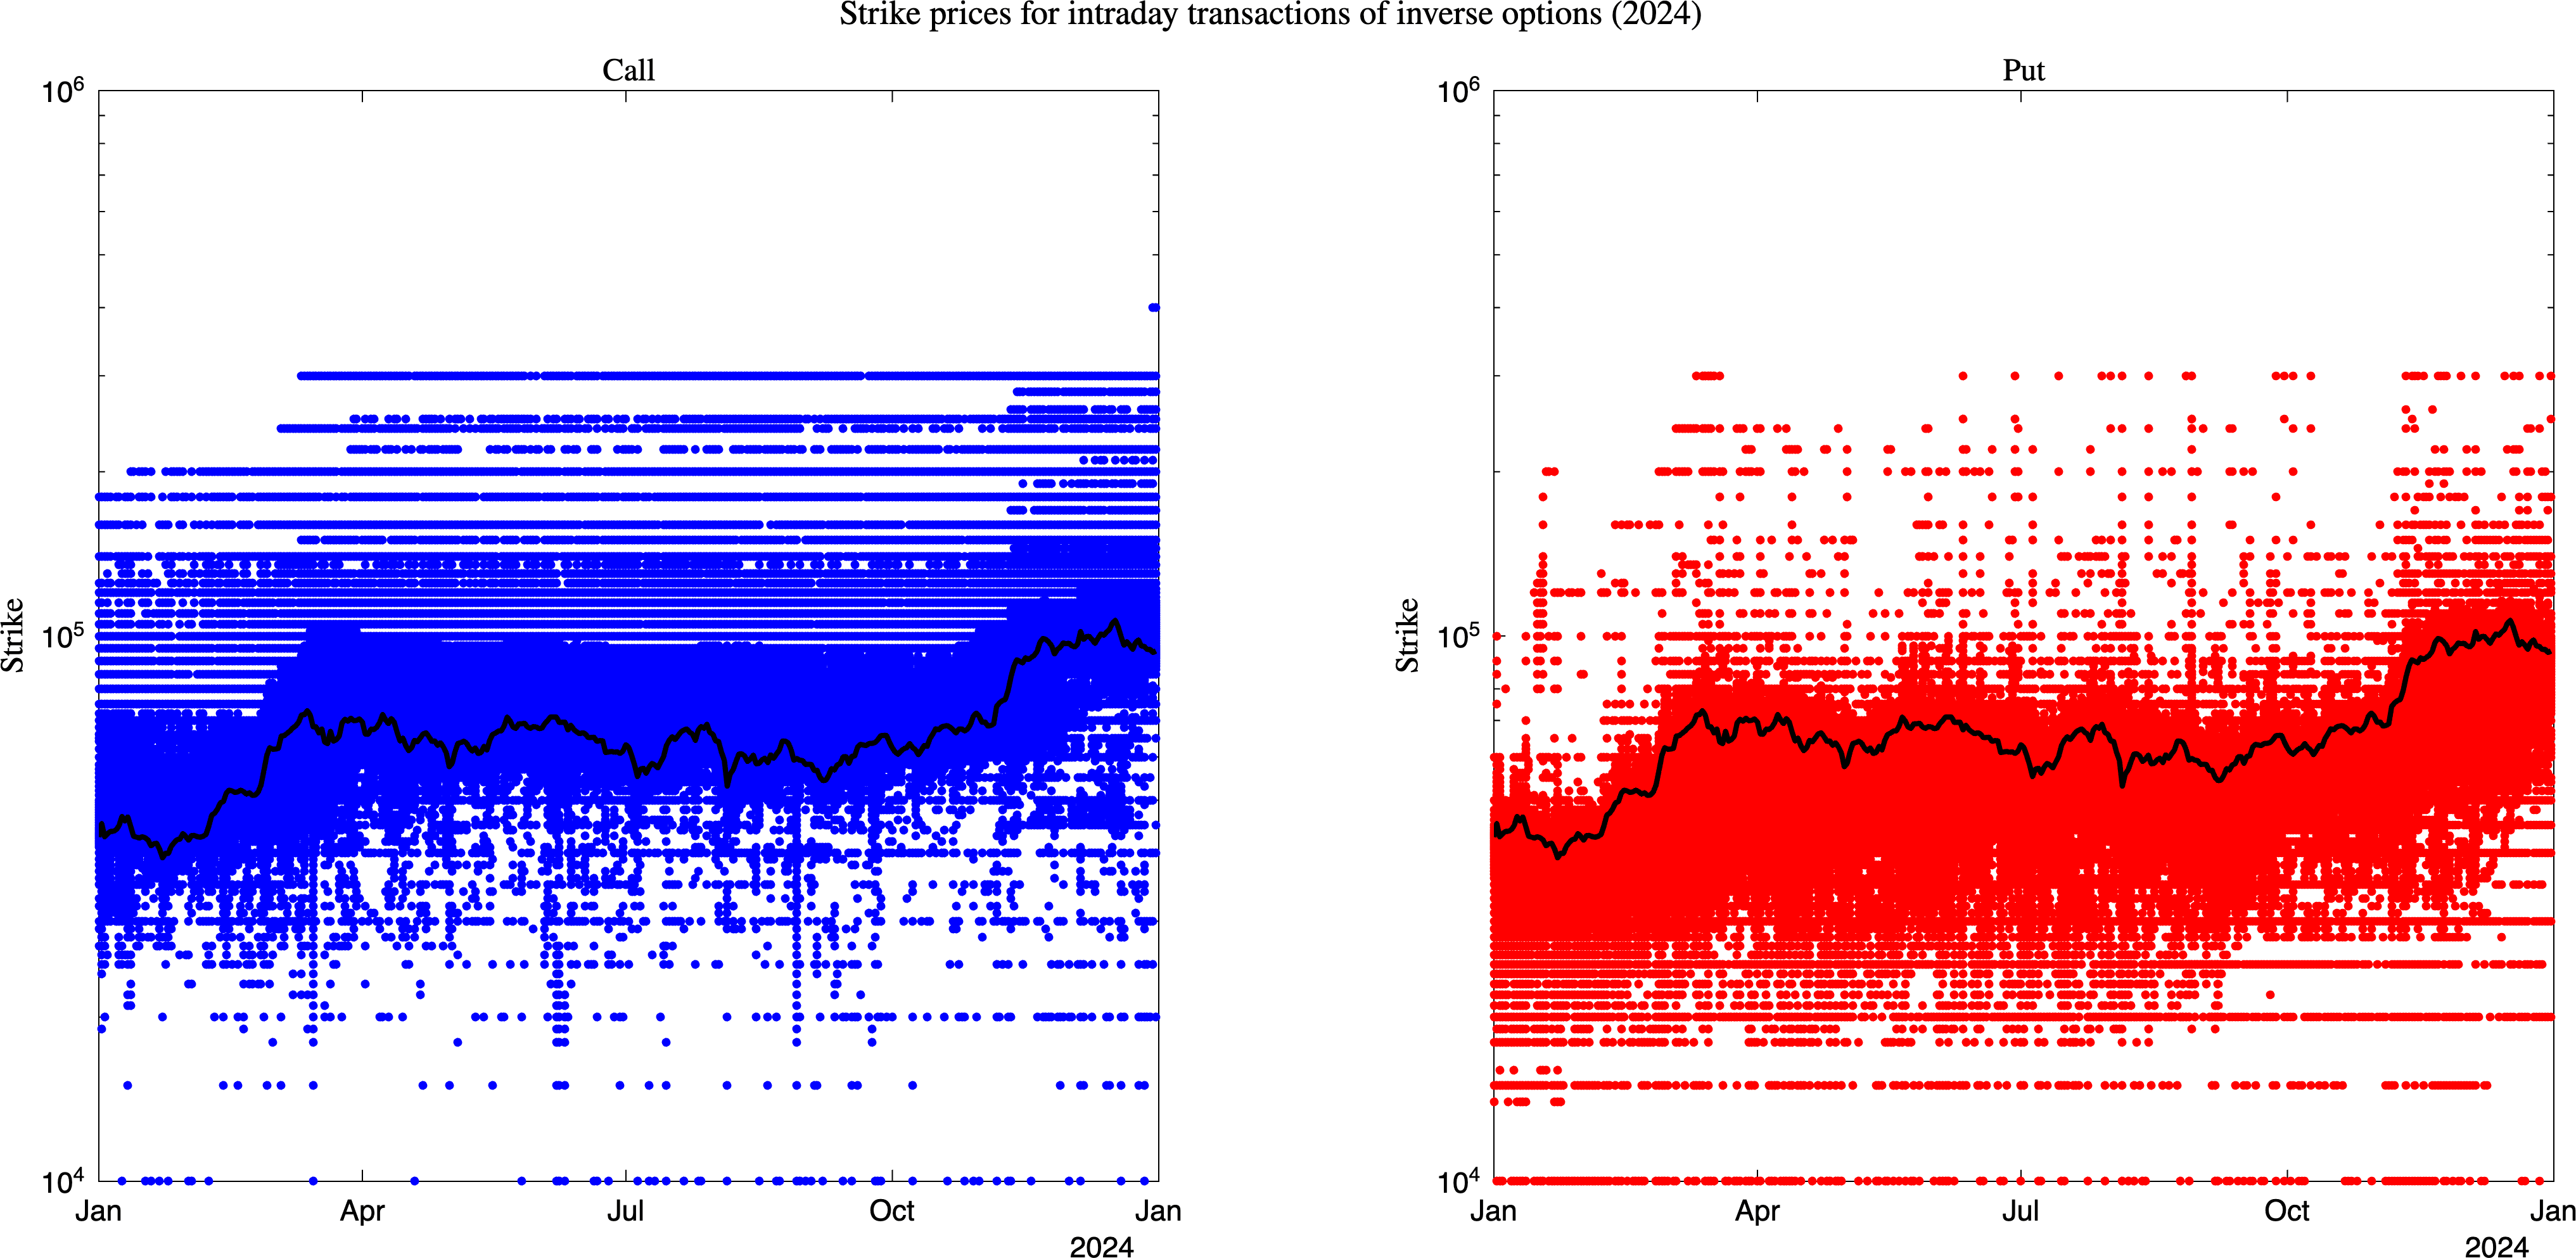
\includegraphics[width=\linewidth]{Sections/02_data_figures/Strike price for the intraday of inverse options.png}
    \caption{Visualizing strike prices for the intraday transaction of inverse
options}
    \label{fig:Prices_for_cp}
\end{figure}

Figure~\ref{fig:Prices_for_cp} illustrates the cross-sectional distribution of strike prices across the full year for calls (blue) and puts (red), with the black line tracing the daily spot price. Strikes span more than two orders of magnitude on a logarithmic scale – from approximately \$10,000 to \$1,000,000 – with the densest concentration in a band surrounding the at-the-money level, confirming that the most actively traded contracts are near-the-money options. The upward drift of the strike distribution mirrors the appreciation of the underlying spot price, indicating that market participants continuously recalibrate their hedging and speculative positions as BTC's price evolves.


For each UTC date and each instrument, let $\mathcal{I}_{j,d}(h)$ denote the set of eligible trades in the interval $[08{:}00-h,08{:}00+h]$, where $h$ is the half-window width. Liquidations, combination-strategy legs, block trades, and RFQ (Request for Quote) trades are excluded. The baseline closing price is the eligible trade closest to 08:00,
\begin{equation}
 p^{\mathrm{close}}_{j,d}
 =p_{i^{*},j,d}, \qquad
 i^{*}=\arg\min_{i\in\mathcal{I}_{j,d}(h)}
 \left|t_{i,j,d}-08{:}00\right|.
 \label{eq:closest_closing_trade}
\end{equation}
If multiple transactions are equally close, the larger transaction is selected, followed by the larger trade identifier as a deterministic tie-breaker. We also retain the quantity-weighted average price,
\begin{equation}
 p^{\mathrm{VWAP}}_{j,d}(h)
 =\frac{\sum_{i\in\mathcal{I}_{j,d}(h)}p_{i,j,d}q_{i,j,d}}
 {\sum_{i\in\mathcal{I}_{j,d}(h)}q_{i,j,d}},
 \label{eq:closing_vwap}
\end{equation}
and the median transaction price for robustness analysis. This panel is not an order-book snapshot: contracts without a qualifying transaction are not imputed.

Table~\ref{tab:closing_window_comparison_15min} compares 08:00-centered bandwidths from one to thirty minutes. Wider windows increase the number of available date--contract observations, but also move the selected trade farther from the target valuation time. The 15-minute half-window provides a practical compromise: it increases annual coverage from 27,018 observations under the five-minute window to 46,788 observations, and it captures a meaningfully broader set of longer-maturity contracts while retaining a tight 30-minute calendar window around the settlement time. We therefore use the 15-minute filtered panel as the experimental option dataset.

\begin{figure}[h]
    \centering
    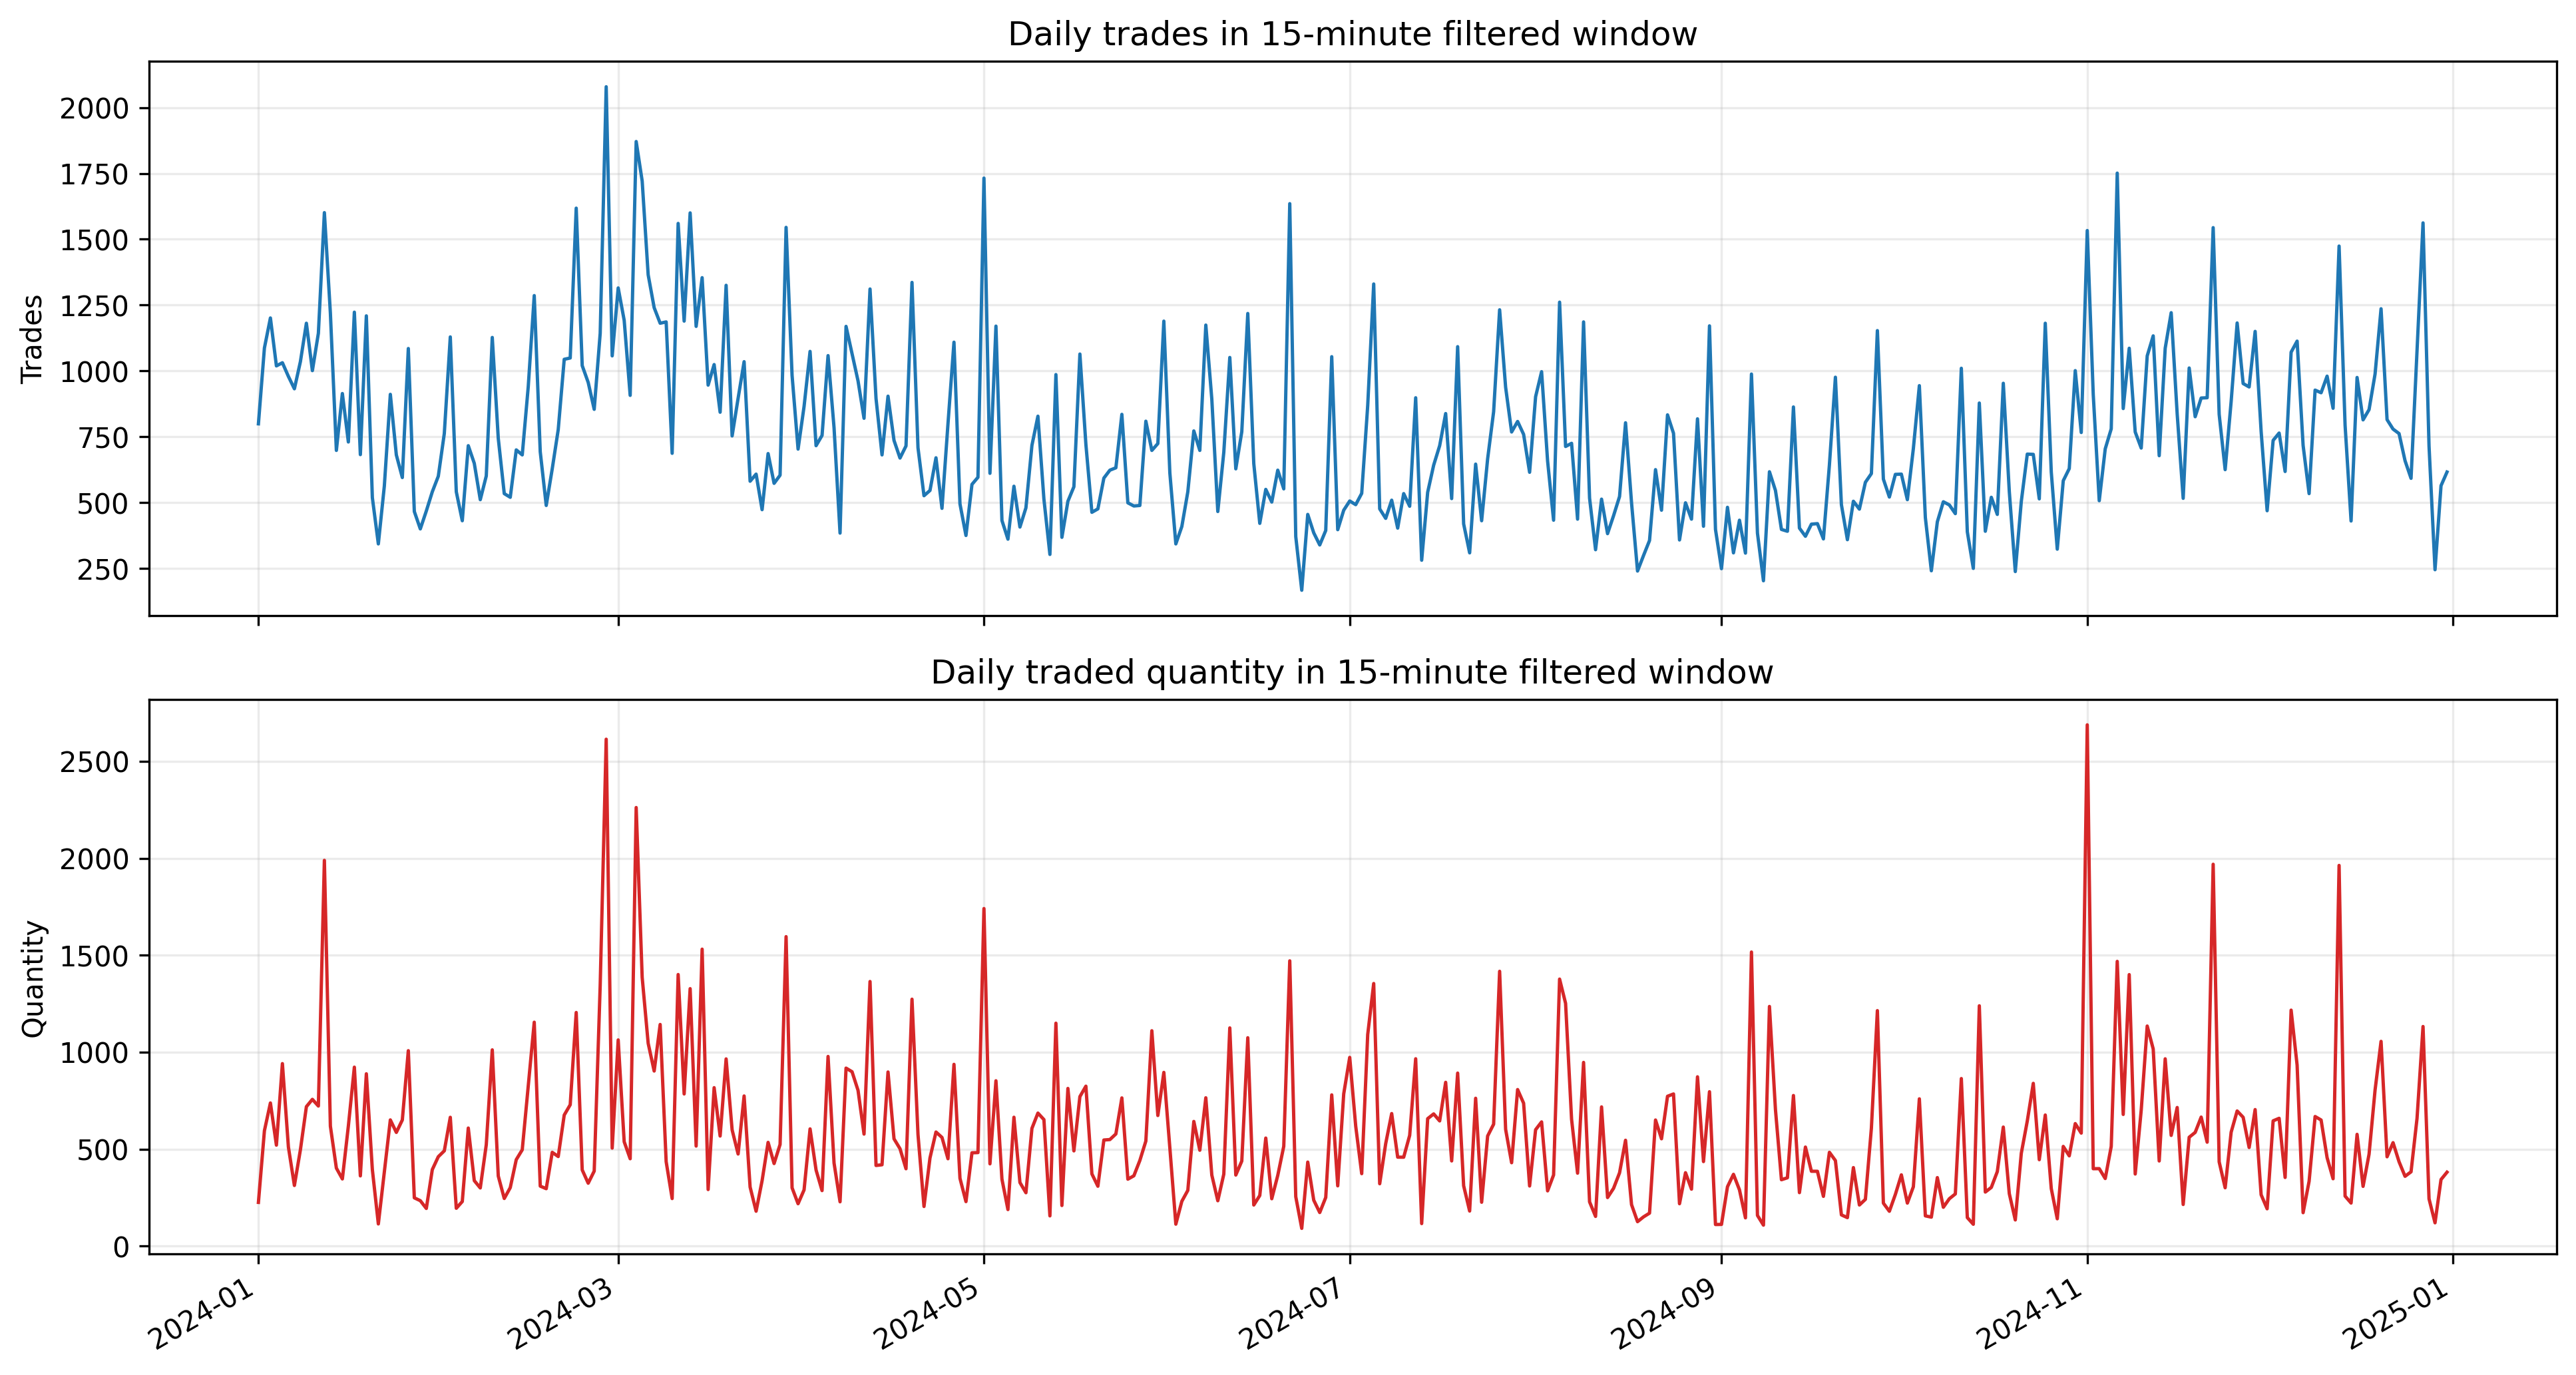
\includegraphics[width=\linewidth]{Sections/02_data_figures/Daily_traded_quantity_15min_filtered.png}
    \caption{Daily accumulated trades and quantities in the 15-minute filtered Deribit BTC inverse option panel}
    \label{fig:daily_quantity_15min_filtered}
\end{figure}

Figure~\ref{fig:daily_quantity_15min_filtered} shows trading activity inside the 15-minute closing window. The number of trades and total quantity vary substantially over time, with visible bursts around periods of elevated Bitcoin market activity. Since each retained date--contract observation is constructed from actual transactions near 08:00 UTC, the panel balances contemporaneous cross-sectional pricing with sufficient coverage for daily calibration.

\begin{figure}[h]
    \centering
    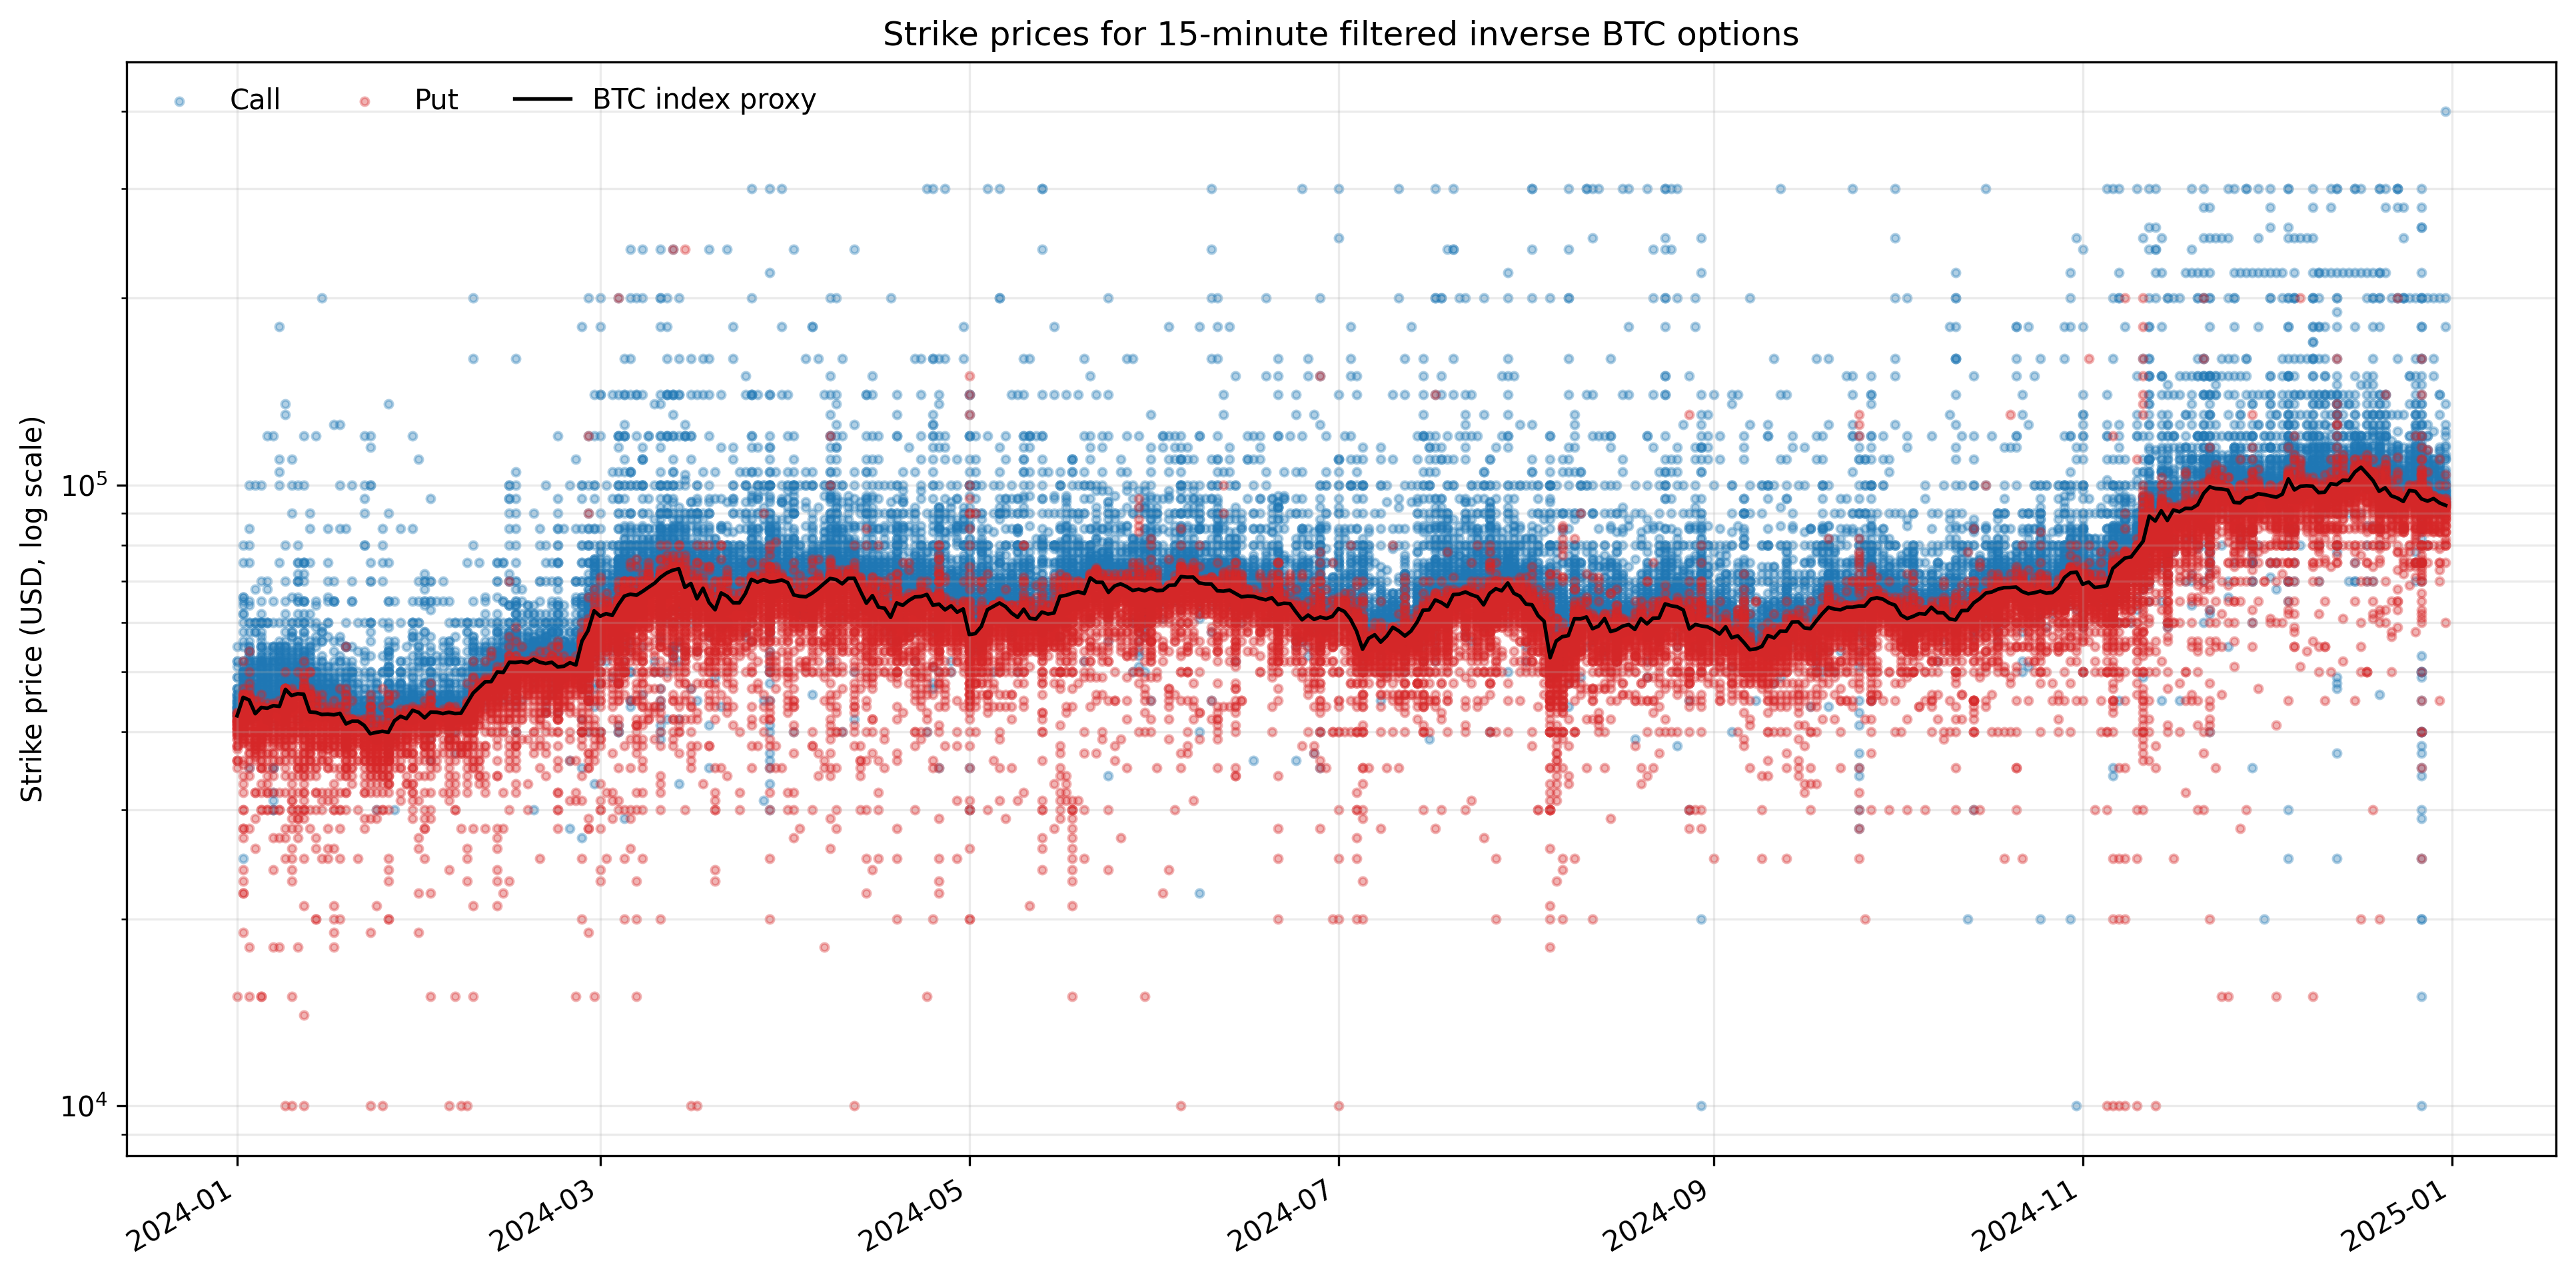
\includegraphics[width=\linewidth]{Sections/02_data_figures/Strike_price_15min_filtered_inverse_options.png}
    \caption{Visualizing strike prices for 15-minute filtered inverse BTC option observations}
    \label{fig:strike_15min_filtered}
\end{figure}

Figure~\ref{fig:strike_15min_filtered} displays the strike distribution of the filtered panel, with calls and puts shown separately and the 08:00 BTC index-price proxy overlaid in black. The filtered sample preserves a wide cross-section of strikes around the money while also retaining far out-of-the-money observations in both tails.

All maturity-related tables below use accurate time to maturity, measured from the selected transaction timestamp to the contract expiration timestamp. Thus an option traded exactly at 08:00 UTC one day before expiration has $T=1$, while a trade at 20:00 UTC one day before expiration would have $T=0.5$. In the 15-minute filtered panel this correction is small but conceptually important because the retained transaction need not occur exactly at 08:00.

\begin{table}[htbp]
\centering
\caption{\textbf{Comparison of daily closing-price windows.} For every UTC date in 2024, the table summarizes eligible regular outright BTC inverse-option transactions in a window centered on 08:00 UTC. Daily instruments counts distinct contracts with at least one eligible trade, and annual observations counts unique date--instrument pairs.}
\label{tab:closing_window_comparison_15min}
\begin{tabular}{lrrrrrr}
\toprule
Half-window & Full window & \multicolumn{2}{c}{Daily trades} & \multicolumn{2}{c}{Daily instruments} & Annual\\
\cmidrule(lr){3-4}\cmidrule(lr){5-6}
$h$ & width & Mean & Median & Mean & Median & observations\\
\midrule
$\pm 1$ min & 2 min & 52.76 & 45 & 22.27 & 21 & 8,151 \\
$\pm 2$ min & 4 min & 145.07 & 131 & 42.46 & 38 & 15,541 \\
$\pm 5$ min & 10 min & 411.99 & 366 & 73.82 & 66 & 27,018 \\
$\pm 10$ min & 20 min & 607.66 & 557 & 105.27 & 96 & 38,528 \\
$\pm 15$ min & 30 min & 756.87 & 698 & 127.84 & 118 & 46,788 \\
$\pm 20$ min & 40 min & 895.96 & 819 & 146.49 & 137 & 53,616 \\
$\pm 30$ min & 60 min & 1151.52 & 1034 & 176.33 & 166 & 64,537 \\
\bottomrule
\end{tabular}
\end{table}


\begin{table}[h]
\centering
\caption{\textbf{Distributions of 15-minute filtered option characteristics}. The table presents percentiles for BTC call and put options' accurate time to maturity ($T$), moneyness ($S_0/K$), and closest transaction prices ($p$).}
\label{tab:filtered_option_characteristics}
\begin{tabular}{lrrrrrr}
\hline
 & \multicolumn{2}{c}{T} & \multicolumn{2}{c}{S0/K} & \multicolumn{2}{c}{p} \\
 & Call & Put & Call & Put & Call & Put \\
\hline
Min & 0.00 & 0.00 & 0.19 & 0.29 & 0.0001 & 0.0001 \\
$Q_1$ & 0.00 & 0.00 & 0.40 & 0.87 & 0.0001 & 0.0001 \\
$Q_5$ & 1.00 & 1.00 & 0.65 & 0.96 & 0.0002 & 0.0002 \\
$Q_{10}$ & 1.00 & 1.00 & 0.75 & 0.98 & 0.0003 & 0.0003 \\
$Q_{20}$ & 1.01 & 1.00 & 0.85 & 1.00 & 0.0011 & 0.0010 \\
$Q_{30}$ & 2.00 & 2.00 & 0.89 & 1.02 & 0.0027 & 0.0021 \\
$Q_{40}$ & 3.00 & 2.01 & 0.92 & 1.03 & 0.0055 & 0.0041 \\
$Q_{50}$ & 7.00 & 4.99 & 0.94 & 1.05 & 0.0095 & 0.0075 \\
$Q_{60}$ & 12.00 & 8.99 & 0.96 & 1.08 & 0.0155 & 0.0120 \\
$Q_{70}$ & 18.01 & 14.01 & 0.98 & 1.10 & 0.0255 & 0.0195 \\
$Q_{80}$ & 35.00 & 25.00 & 0.99 & 1.15 & 0.0420 & 0.0325 \\
$Q_{90}$ & 72.00 & 56.99 & 1.01 & 1.27 & 0.0750 & 0.0580 \\
$Q_{95}$ & 122.99 & 88.99 & 1.05 & 1.44 & 0.1160 & 0.0895 \\
$Q_{99}$ & 291.51 & 254.00 & 1.26 & 2.16 & 0.2585 & 0.1835 \\
$Q_{99.9}$ & 356.99 & 351.72 & 2.41 & 4.46 & 0.6140 & 0.7303 \\
$Q_{99.99}$ & 364.00 & 362.00 & 6.14 & 7.60 & 0.8379 & 1.7365 \\
Max & 364.01 & 364.00 & 9.50 & 8.75 & 0.8960 & 2.1050 \\
\hline
\end{tabular}
\end{table}


Tables 2 and 3 report the same three characteristics - time to maturity ($T$), moneyness ($S_0/K$), and price ($p$) - but Table \ref{tab:weighted_option_characteristics} reweights each contract by traded volume rather than treating each observation equally. The comparison reveals a systematic shift in the bulk of the distribution once size is accounted for, while the extreme tails remain essentially unchanged.

For maturity, the weighted median maturity roughly doubles relative to the unweighted median (calls: 7 $\to$ 14 days; puts: 4 $\to$ 9 days), and this pattern persists through the 90th percentile (calls: 65 $\to$ 98; puts: 50 $\to$ 65). This indicates that larger trades are disproportionately concentrated in longer-dated contracts, rather than in the very short-dated options that dominate the raw contract count.

For moneyness, volume-weighting pulls the put-side distribution further out-of-the-money - the $Q_{90}$ for puts rises from 1.22 to 1.29 and $Q_{95}$
from 1.36 to 1.45 - while the call side is little changed or slightly more concentrated near-the-money at the median (0.96 $\to$ 0.93). This asymmetry is consistent with large-size trading activity being driven by downside/tail-hedging demand rather than symmetric directional speculation.

For price, reflecting both the longer maturities and deeper OTM put skew, weighted median prices are noticeably higher (calls: 0.0105 $\to$ 0.0162; puts: 0.0079 $\to$ 0.0105 BTC).

Notably, the extreme upper tail ($Q_{99.9}$ and beyond) is nearly identical across both tables for all three characteristics, since these percentiles are anchored by the same small set of extreme contracts regardless of weighting. The divergence is therefore a genuine feature of the bulk of the distribution, not an artifact of outliers - a useful diagnostic if you weight your Q-calibration loss function by trade size, since doing so will implicitly shift emphasis toward longer-dated, more OTM put contracts relative to an unweighted (per-contract) loss.


\begin{table}[h]
\centering
\caption{\textbf{Quantity-weighted distributions of 15-minute filtered option characteristics}. Percentiles are weighted by total contract quantity in each 15-minute window.}
\label{tab:filtered_weighted_option_characteristics}
\begin{tabular}{lrrrrrr}
\hline
 & \multicolumn{2}{c}{T} & \multicolumn{2}{c}{S0/K} & \multicolumn{2}{c}{p} \\
 & Call & Put & Call & Put & Call & Put \\
\hline
Min & 0.00 & 0.00 & 0.19 & 0.29 & 0.0001 & 0.0001 \\
$Q_1$ & 0.01 & 0.01 & 0.43 & 0.92 & 0.0001 & 0.0001 \\
$Q_5$ & 1.00 & 1.00 & 0.66 & 0.98 & 0.0002 & 0.0002 \\
$Q_{10}$ & 1.00 & 1.00 & 0.76 & 1.00 & 0.0004 & 0.0004 \\
$Q_{20}$ & 1.00 & 1.00 & 0.86 & 1.01 & 0.0013 & 0.0009 \\
$Q_{30}$ & 1.00 & 1.00 & 0.90 & 1.02 & 0.0029 & 0.0018 \\
$Q_{40}$ & 2.00 & 2.00 & 0.93 & 1.03 & 0.0050 & 0.0035 \\
$Q_{50}$ & 5.99 & 3.00 & 0.95 & 1.05 & 0.0080 & 0.0055 \\
$Q_{60}$ & 8.00 & 7.00 & 0.97 & 1.07 & 0.0120 & 0.0085 \\
$Q_{70}$ & 14.99 & 10.00 & 0.98 & 1.10 & 0.0180 & 0.0125 \\
$Q_{80}$ & 25.00 & 18.99 & 0.99 & 1.15 & 0.0300 & 0.0215 \\
$Q_{90}$ & 56.00 & 45.00 & 1.00 & 1.29 & 0.0525 & 0.0410 \\
$Q_{95}$ & 103.00 & 72.00 & 1.02 & 1.44 & 0.0810 & 0.0655 \\
$Q_{99}$ & 242.00 & 190.01 & 1.12 & 2.56 & 0.1785 & 0.1350 \\
$Q_{99.9}$ & 343.01 & 326.99 & 1.75 & 7.34 & 0.4595 & 0.2830 \\
$Q_{99.99}$ & 360.99 & 362.00 & 7.24 & 8.75 & 0.8645 & 0.6345 \\
Max & 364.01 & 364.00 & 9.50 & 8.75 & 0.8960 & 2.1050 \\
\hline
\end{tabular}
\caption{\textbf{Weighted distributions of option characteristics}. The table presents percentiles for BTC call and put options' time to maturity ($T$), moneyness ($S_0/K$), and prices ($p$), with $Q_k$ representing the $k$-th percentile.}
\label{tab:weighted_option_characteristics}
\end{table}


\begin{table}[h]
\centering
\caption{\textbf{Maturity-moneyness categories for 15-minute filtered options}. The table reports the proportion (\%) of date--contract observations in each category.}
\label{tab:filtered_maturity_moneyness_categories}
\begin{tabular}{lrrrr}
\hline
Inverse BTC call option & Deep OTM & OTM & ITM & \\
 & $\frac{S_0}{K} \leq 0.86$ & $0.86 < \frac{S_0}{K} \leq 1$ & $1 < \frac{S_0}{K}$ & Sum \\
\hline
Short-term: $T \leq 7$ & 1.5\% & 21.5\% & 4.2\% & 27.1\% \\
Mid-term: $7 < T \leq 28$ & 3.4\% & 8.0\% & 2.3\% & 13.7\% \\
Long-term: $28 < T$ & 6.7\% & 3.9\% & 1.4\% & 11.9\% \\
Sum & 11.5\% & 33.3\% & 7.9\% & 52.7\% \\
\hline
Inverse BTC put option & ITM & OTM & Deep OTM & \\
 & $\frac{S_0}{K} \leq 1$ & $1 < \frac{S_0}{K} \leq 1.12$ & $1.12 < \frac{S_0}{K}$ & Sum \\
\hline
Short-term: $T \leq 7$ & 4.5\% & 19.0\% & 3.4\% & 27.0\% \\
Mid-term: $7 < T \leq 28$ & 2.2\% & 5.3\% & 4.0\% & 11.4\% \\
Long-term: $28 < T$ & 1.7\% & 2.4\% & 4.9\% & 9.0\% \\
Sum & 8.3\% & 26.7\% & 12.3\% & 47.3\% \\
\hline
\end{tabular}
\end{table}

Tables \ref{tab:maturity_moneyness_categories} and \ref{tab:weighted_maturity_moneyness_categories} partition trading activity into a 3$\times$3 maturity-moneyness grid for calls and puts separately, contrasting the raw trade-count distribution (Table \ref{tab:maturity_moneyness_categories}) with the quantity-weighted distribution (Table \ref{tab:weighted_maturity_moneyness_categories}). Two consistent patterns emerge once volume is used as the weight instead of trade count.

Shift from short-term to long-term. Under the unweighted count, short-term options ($T\le 7$) dominate both calls (28.6\%) and puts (26.1\%), while long-term options are the smallest bucket (11.8\% calls, 7.7\% puts). Weighting by quantity essentially reverses this ordering for calls: long-term rises to 20.5\%, roughly matching short-term's 21.7\%, while for puts the short-term share nearly halves (26.1\% $\to$ 17.6\%) and long-term rises modestly (7.7\% $\to$ 9.7\%). This confirms what Table \ref{tab:weighted_option_characteristics} already suggested from the marginal maturity distribution — large trades cluster in longer-dated contracts, so a small number of big long-dated trades can rival a much larger number of small short-dated ones.

Shift toward deep OTM, especially at long maturities. The clearest movement is in the OTM/deep-OTM composition. For calls, deep-OTM share more than doubles for the long-term bucket alone (6.4\% $\to$ 12.4\%), and the overall call deep-OTM sum rises from 10.0\% to 17.1\%. For puts, the deep-OTM long-term cell rises from 4.2\% to 5.6\%, and overall put deep-OTM rises from 9.8\% to 11.8\%, while the near-the-money OTM bucket shrinks correspondingly (put OTM sum: 29.0\% → 22.6\%). This is consistent with the earlier percentile analysis: large trades skew toward tail hedges rather than near-the-money speculative flow.

Calls vs. puts asymmetry persists. Across both weighting schemes, calls retain a higher overall trading share than puts (55.1\% vs. 44.9\% unweighted; 60.6\% vs. 39.4\% weighted), and this gap widens under volume weighting — implying call-side activity is not just more frequent but carried out in larger size, plausibly reflecting basis-trade or covered-call-type flow that's naturally larger in inverse (BTC-margined) contracts.


\begin{table}[h]
\centering
\caption{\textbf{Quantity-weighted maturity-moneyness categories for 15-minute filtered options}. The table reports the proportion (\%) of total 15-minute window quantity in each category.}
\label{tab:filtered_weighted_maturity_moneyness_categories}
\begin{tabular}{lrrrr}
\hline
Inverse BTC call option & Deep OTM & OTM & ITM & \\
 & $\frac{S_0}{K} \leq 0.86$ & $0.86 < \frac{S_0}{K} \leq 1$ & $1 < \frac{S_0}{K}$ & Sum \\
\hline
Short-term: $T \leq 7$ & 1.6\% & 26.9\% & 3.3\% & 31.9\% \\
Mid-term: $7 < T \leq 28$ & 3.6\% & 8.8\% & 2.0\% & 14.5\% \\
Long-term: $28 < T$ & 6.6\% & 3.0\% & 0.7\% & 10.3\% \\
Sum & 11.8\% & 38.8\% & 6.1\% & 56.7\% \\
\hline
Inverse BTC put option & ITM & OTM & Deep OTM & \\
 & $\frac{S_0}{K} \leq 1$ & $1 < \frac{S_0}{K} \leq 1.12$ & $1.12 < \frac{S_0}{K}$ & Sum \\
\hline
Short-term: $T \leq 7$ & 3.2\% & 21.0\% & 3.5\% & 27.7\% \\
Mid-term: $7 < T \leq 28$ & 1.5\% & 4.2\% & 3.6\% & 9.3\% \\
Long-term: $28 < T$ & 0.9\% & 1.5\% & 3.9\% & 6.3\% \\
Sum & 5.6\% & 26.6\% & 11.1\% & 43.3\% \\
\hline
\end{tabular}
\caption{\textbf{Weighted Maturity-moneyness categories}. The table delineates nine categories based on maturity-moneyness. Short-term, mid-term, and long-term options are defined by $T \leq 7$, $7 < T \leq 28$, and $28 < T$, while OTM, ITM, and deep OTM options are defined by their moneyness ($S_0/K$). The table reports the proportion (\%) of trades in each maturity-moneyness category.}
\label{tab:weighted_maturity_moneyness_categories}
\end{table}

\begin{table}[h]
\centering
\caption{\textbf{Average prices in BTC and standard deviations for 15-minute filtered inverse options}. Standard deviations are in parentheses.}
\label{tab:filtered_average_prices_inverse_options}
\begin{tabular}{lccc}
\hline
Inverse BTC call option & Deep OTM & OTM & ITM \\
 & $\frac{S_0}{K} \leq 0.86$ & $0.86 < \frac{S_0}{K} \leq 1$ & $1 < \frac{S_0}{K}$ \\
\hline
Short-term: $T \leq 7$ & \makecell{0.0006\\(0.0008)} & \makecell{0.0045\\(0.0057)} & \makecell{0.0449\\(0.0694)} \\
Mid-term: $7 < T \leq 28$ & \makecell{0.0042\\(0.0045)} & \makecell{0.0228\\(0.0148)} & \makecell{0.0862\\(0.0742)} \\
Long-term: $28 < T$ & \makecell{0.0373\\(0.0422)} & \makecell{0.0794\\(0.0477)} & \makecell{0.2075\\(0.1449)} \\
\hline
Inverse BTC put option & ITM & OTM & Deep OTM \\
 & $\frac{S_0}{K} \leq 1$ & $1 < \frac{S_0}{K} \leq 1.12$ & $1.12 < \frac{S_0}{K}$ \\
\hline
Short-term: $T \leq 7$ & \makecell{0.0353\\(0.0551)} & \makecell{0.0045\\(0.0054)} & \makecell{0.0008\\(0.0012)} \\
Mid-term: $7 < T \leq 28$ & \makecell{0.0694\\(0.0554)} & \makecell{0.0219\\(0.0118)} & \makecell{0.0043\\(0.0040)} \\
Long-term: $28 < T$ & \makecell{0.1696\\(0.2020)} & \makecell{0.0617\\(0.0291)} & \makecell{0.0214\\(0.0225)} \\
\hline
\end{tabular}
\end{table}

\begin{table}[h]
\centering
\caption{\textbf{Quantity-weighted average prices in BTC and standard deviations for 15-minute filtered inverse options}. Weighted standard deviations are in parentheses.}
\label{tab:filtered_weighted_average_prices_inverse_options}
\begin{tabular}{lccc}
\hline
Inverse BTC call option & Deep OTM & OTM & ITM \\
 & $\frac{S_0}{K} \leq 0.86$ & $0.86 < \frac{S_0}{K} \leq 1$ & $1 < \frac{S_0}{K}$ \\
\hline
Short-term: $T \leq 7$ & \makecell{0.0005\\(0.0009)} & \makecell{0.0052\\(0.0060)} & \makecell{0.0303\\(0.0437)} \\
Mid-term: $7 < T \leq 28$ & \makecell{0.0058\\(0.0062)} & \makecell{0.0213\\(0.0142)} & \makecell{0.0778\\(0.0567)} \\
Long-term: $28 < T$ & \makecell{0.0334\\(0.0374)} & \makecell{0.0722\\(0.0446)} & \makecell{0.1976\\(0.1525)} \\
\hline
Inverse BTC put option & ITM & OTM & Deep OTM \\
 & $\frac{S_0}{K} \leq 1$ & $1 < \frac{S_0}{K} \leq 1.12$ & $1.12 < \frac{S_0}{K}$ \\
\hline
Short-term: $T \leq 7$ & \makecell{0.0275\\(0.0268)} & \makecell{0.0050\\(0.0053)} & \makecell{0.0008\\(0.0012)} \\
Mid-term: $7 < T \leq 28$ & \makecell{0.0645\\(0.0333)} & \makecell{0.0217\\(0.0123)} & \makecell{0.0037\\(0.0038)} \\
Long-term: $28 < T$ & \makecell{0.1347\\(0.1054)} & \makecell{0.0592\\(0.0304)} & \makecell{0.0172\\(0.0177)} \\
\hline
\end{tabular}
\caption{\textbf{Weighted average prices in BTC and standard deviations of inverse options.} This table displays the mean prices and standard deviations in parentheses for options across each maturity-moneyness category.}
\label{tab:weighted_average_prices_inverse_options}
\end{table}

Tables \ref{tab:average_prices_inverse_options} and \ref{tab:weighted_average_prices_inverse_options} report mean BTC-denominated prices (with standard deviations) across the same nine maturity-moneyness buckets, unweighted per-contract versus weighted by traded quantity. Three patterns stand out.

Monotonicity confirms internal consistency. Within both tables, prices rise monotonically with maturity for every moneyness bucket (as expected from time value), and rise monotonically with moneyness for calls (deep OTM cheapest, ITM most expensive) while falling monotonically with moneyness for puts. This is a useful sanity check: the data respects basic no-arbitrage ordering before any model fitting is applied, so any monotonicity violations you find later in the pricing kernel estimate can't be traced back to a raw data pathology at this level.

Weighting effects are asymmetric and bucket-specific, not uniform. Rather than a systematic upward or downward shift, quantity-weighting moves prices in different directions depending on the cell. Sh4ort-term ITM calls are notably more expensive when weighted (0.0326 → 0.0415), suggesting large trades in that bucket occurred disproportionately during high-price/high-vol windows. Conversely, long-term ITM puts are substantially cheaper when weighted (0.1761 → 0.1366) and long-term ITM calls slightly cheaper (0.1873 → 0.1787), suggesting the largest long-dated trades cluster in calmer pricing environments than the per-contract average implies. This bucket-dependent divergence means a single "volume-weighting effect" can't be assumed uniformly across your calibration grid — it needs to be checked cell by cell.

Dispersion is highest exactly where large trades concentrate. The standard deviations are large relative to the means in the long-term ITM buckets — long-term ITM puts show a standard deviation (0.2642 unweighted) that actually exceeds the mean (0.1761), a coefficient of variation above 1. Long-term deep-OTM calls show similar relative dispersion (0.0414 vs. mean 0.0374). Given that Tables 4–5 showed these same long-term/deep buckets are exactly where quantity-weighting shifts trading share upward, this dispersion is plausibly driven by the discrete macro-jump episodes (March, August, November) identified earlier — large trades executed in these buckets during the year likely span both pre- and post-jump price regimes, inflating within-bucket variance.

\clearpage

\subsection{Construction of Daily Closing Option Prices}
\label{subsec:daily_closing_prices}

Daily risk-neutral calibration requires a cross-section of option prices that refers, as closely as the data permit, to a common valuation time. If all transactions over a 24-hour period were pooled into one daily cross-section, differences across strikes and maturities would be confounded by intraday changes in the Bitcoin index, the implied-volatility state, and time to maturity. The resulting collection of prices would therefore not represent the option surface prevailing at any particular instant. This timing consideration is important for option-implied risk-neutral estimation, which treats prices across strikes as a contemporaneous cross-section \citep{AitSahaliaLo1998}. Recent empirical work on Bitcoin risk premia likewise illustrates the use of transaction-level option records organized at a daily frequency \citep{AlmeidaGrithMiftachovWang2024}.

We anchor the daily cross-section at 08:00 UTC. This is the natural boundary of a Deribit trading day: Deribit performs its daily settlement at 08:00 UTC, and its inverse BTC options expire at that time \citep{DeribitSettlement2026}. Exact 08:00 transaction prices are generally unavailable because an option contract need not trade at that instant. We consequently construct a daily closing transaction panel from actual outright trades observed in a short interval centered on 08:00 UTC. This panel should not be interpreted as a synchronous order-book snapshot: contracts without a qualifying transaction are not imputed, and historical bid and ask quotations are not used.

For each UTC date and each instrument, let $\mathcal{I}_{j,d}(h)$ denote the set of eligible trades in the interval $[08{:}00-h,08{:}00+h]$, where $h$ is the half-window width. Liquidations, combination-strategy legs, block trades, and RFQ (Request for quote) trades are excluded so that the retained observations represent regular outright market transactions. Our baseline closing price is the price of the eligible trade closest to 08:00,
\begin{equation}
 p^{\mathrm{close}}_{j,d}
 =p_{i^{*},j,d}, \qquad
 i^{*}=\arg\min_{i\in\mathcal{I}_{j,d}(h)}
 \left|t_{i,j,d}-08{:}00\right|.
 \label{eq:closest_closing_trade}
\end{equation}
If multiple transactions are equally close, the larger transaction is selected, followed by the larger trade identifier as a deterministic tie-breaker. To assess sensitivity to individual prints and bid--ask bounce, we also retain the quantity-weighted average price
\begin{equation}
 p^{\mathrm{VWAP}}_{j,d}(h)
 =\frac{\sum_{i\in\mathcal{I}_{j,d}(h)}p_{i,j,d}q_{i,j,d}}
 {\sum_{i\in\mathcal{I}_{j,d}(h)}q_{i,j,d}},
 \label{eq:closing_vwap}
\end{equation}
and the median transaction price for robustness analysis. Prices are preserved in their original BTC units. USD-equivalent prices are recorded separately by multiplying the BTC premium by the contemporaneous Deribit BTC index; this conversion changes the unit of account but does not transform an asynchronous trade into an exact 08:00 price.

Table~\ref{tab:closing_window_comparison} reports the coverage obtained from half-windows of one, two, and five minutes. The sample contains a qualifying transaction on every one of the 366 calendar days for all three specifications. A one-minute half-window produces only 22.27 distinct instruments per day on average, whereas a five-minute half-window increases average daily coverage to 73.82 instruments and yields 27,018 date--instrument observations over the year. The five-minute half-window, corresponding to 07:55--08:05 UTC, is therefore used to construct the preliminary closing panel. The closest-transaction price remains the baseline measure, while the five-minute VWAP and median price are retained for robustness checks. The shorter windows will be used to assess the sensitivity of the subsequent calibration to the trade-off between temporal synchronization and cross-sectional coverage.

\begin{table}[htbp]
\centering
\begin{tabular}{lrrrrrr}
\toprule
Half-window & Full window & \multicolumn{2}{c}{Daily trades} & \multicolumn{2}{c}{Daily instruments} & Annual\\
\cmidrule(lr){3-4}\cmidrule(lr){5-6}
$h$ & width & Mean & Median & Mean & Median & observations\\
\midrule
$\pm 1$ minute  & 2 minutes  & 52.76  & 45  & 22.27 & 21 & 8,151\\
$\pm 2$ minutes & 4 minutes  & 145.07 & 131 & 42.46 & 38 & 15,541\\
$\pm 5$ minutes & 10 minutes & 411.99 & 366 & 73.82 & 66 & 27,018\\
\bottomrule
\end{tabular}
\caption{\textbf{Comparison of daily closing-price windows.} For every UTC date in 2024, the table summarizes eligible regular outright BTC inverse-option transactions in a window centered on 08:00 UTC. ``Daily instruments'' counts distinct contracts with at least one eligible trade, and ``Annual observations'' counts unique date--instrument pairs. Liquidations, combination-strategy legs, block trades, and RFQ trades are excluded. All three windows contain at least one eligible transaction on each of the 366 sample days.}
\label{tab:closing_window_comparison}
\end{table}
\clearpage
